% -----------------------------------------------
% Template for SMC 2022
% based on SMC 2022 template
% -----------------------------------------------

\documentclass{article}
\usepackage{smc}
\usepackage{times}
\usepackage{listings}
\usepackage{ifpdf}
\usepackage[english]{babel}
\usepackage{cite}

\lstdefinestyle{psstyle}{
  basicstyle=\ttfamily\small
}

%%%%%%%%%%%%%%%%%%%%%%%% Some useful packages %%%%%%%%%%%%%%%%%%%%%%%%%%%%%%%
%%%%%%%%%%%%%%%%%%%%%%%% See related documentation %%%%%%%%%%%%%%%%%%%%%%%%%%
%\usepackage{amsmath} % popular packages from Am. Math. Soc. Please use the
%\usepackage{amssymb} % related math environments (split, subequation, cases,
%\usepackage{amsfonts}% multline, etc.)
%\usepackage{bm}      % Bold Math package, defines the command \bf{}
%\usepackage{paralist}% extended list environments
%%subfig.sty is the modern replacement for subfigure.sty. However, subfig.sty
%%requires and automatically loads caption.sty which overrides class handling
%%of captions. To prevent this problem, preload caption.sty with caption=false
%\usepackage[caption=false]{caption}
%\usepackage[font=footnotesize]{subfig}


%user defined variables
\def\papertitle{Zero-cost abstractions to manage audio resource allocation in functional audio languages}
\def\firstauthor{Mike Solomon}

% adds the automatic
% Saves a lot of output space in PDF... after conversion with the distiller
% Delete if you cannot get PS fonts working on your system.

% pdf-tex settings: detect automatically if run by latex or pdflatex
\newif\ifpdf
\ifx\pdfoutput\relax
\else
   \ifcase\pdfoutput
      \pdffalse
   \else
      \pdftrue
\fi

\ifpdf % compiling with pdflatex
  \usepackage[pdftex,
    pdftitle={\papertitle},
    pdfauthor={\firstauthor},
    bookmarksnumbered, % use section numbers with bookmarks
    pdfstartview=XYZ % start with zoom=100% instead of full screen;
                     % especially useful if working with a big screen :-)
   ]{hyperref}
  %\pdfcompresslevel=9

  \usepackage[pdftex]{graphicx}
  % declare the path(s) where your graphic files are and their extensions so
  %you won't have to specify these with every instance of \includegraphics
  \graphicspath{{./figures/}}
  \DeclareGraphicsExtensions{.pdf,.jpeg,.png}

  \usepackage[figure,table]{hypcap}

\else % compiling with latex
  \usepackage[dvips,
    bookmarksnumbered, % use section numbers with bookmarks
    pdfstartview=XYZ % start with zoom=100% instead of full screen
  ]{hyperref}  % hyperrefs are active in the pdf file after conversion

  \usepackage[dvips]{epsfig,graphicx}
  % declare the path(s) where your graphic files are and their extensions so
  %you won't have to specify these with every instance of \includegraphics
  \graphicspath{{./figures/}}
  \DeclareGraphicsExtensions{.eps}

  \usepackage[figure,table]{hypcap}
\fi

%setup the hyperref package - make the links black without a surrounding frame
\hypersetup{
    colorlinks,%
    citecolor=black,%
    filecolor=black,%
    linkcolor=black,%
    urlcolor=black
}


% Title.
% ------
\title{\papertitle}

% Authors
% Please note that submissions are NOT anonymous, therefore
% authors' names have to be VISIBLE in your manuscript.
%
% Single address
% To use with only one author or several with the same address
% ---------------
\oneauthor
   {\firstauthor} {wags.fm \\ %
     {\tt \href{mailto:mike@wavr.so}{mike@wavr.so}}}



% ***************************************** the document starts here ***************
\begin{document}
%
\capstartfalse
\maketitle
\capstarttrue
%
\begin{abstract}
Audio programming languages fall into two broad categories: imperative (CSound, sclang) and functional (Faust, tidal). For the latter, the declarative and immutable nature of data and control structures are often at odds with the mutable and referentially opaque nature of audio units like oscillators and filters. Recently, languages such as Rust have simplified this task through zero-cost abstractions to manage resource allocation in otherwise functional settings. This paper applies these techniques to functional audio programming languages. In addition to correct and low-latency automatic audio memory management, we will see how these techniques allow for efficient namespacing, drastically reducing the amount of time it takes for ceratin graph traversals.
\end{abstract}
%

\section{Introduction}\label{sec:introduction}
The prevailing resource-management paradigm in all modern DAWs and most visual or text-based music creation environments is to model resources as units that are connected to each other. Several examples of this are shown in \ref{fig:audio-units}.

\begin{figure}[t]
\centering
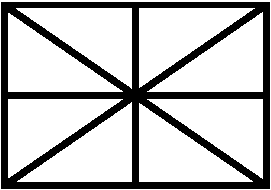
\includegraphics[width=0.6\columnwidth]{figure}
\caption{Figure captions should be placed below the figure,
exactly like this.\label{fig:audio-units}}
\end{figure}

% web audio example
% max example
% supercollider example

Almost all audio units preserve some notion of state internally. For example:

\begin{itemize}
\item Waveforms remember their previous position in a lookup table so that changes in frequency do not disrupt phase.
\item Biquad filters and delay lines need to access a certain number of input samples in the past as well as potentially their own output.
\item FFT-based algorithms need to access and aggregate previous FFTs using a windowing function before rendering the output in the time domain.
\end{itemize}

Because of this, subbing out one audio-unit for another cannot be done in the same way that one would substitute a referrentially transparent value like a floating-point number or boolean. In the most extreme cases, for example with a convolution unit, there are undesirable audio artifacts coupled with seconds of lost rendering data.

In imperative audio programming langauges, such as the Web Audio API or PureData, managing stateful units is a core feature of the language. Variables reference a specific generator that on which arbitrary side effects, like setting a frequency or a volume, can be performed:

%

However, in graph-based langauges, this is more challenging. Consider, for example, the following pseudocode:

\lstset{language=Haskell, style=psstyle}
\begin{lstlisting}
type KPT = { time :: Number, kp :: Boolean }
render :: KPT -> AudioGraph
render { time, kp } =
  (
    if time < 5
    then sinOsc (time * 220)
    else if time < 10
    then sinOsc (time * 50)
    else highpass (playBuf "hello")
  ) <>
  (
    when kp (sinOsc 880)
  )
\end{lstlisting}

We are now demanding much more of the audio engine:
\begin{itemize}
\item Even though we haven't specified it, in almost all circumstances we will want to preserve the sine-wave oscillator across the five-second mark to avoid phase disruption.
\item We do not want the engine to spuriously tear down or create new oscillators, for example arbitrarily changing oscialltor units before the 10-second mark.
\item For precise onsets like a keypress (represented by \texttt{kp}), we want to be as reactive as possible, while at the same time avoiding the creation of an event loop that consumes too much CPU or is so tight that it consistently misses a rendering deadline.
\item We want as little runtime accounting as possible, ideally precompiling an efficient kernel to minimize how much time is spent on our control thread.
\end{itemize}

As graph-based languages such as Tidal Cycles and PureScript Wags become more prevelant, it is important to maintain the helpful abstraction of graphs as a pure function of time while rigorously keeping track of active and inactive audio units with as little computational overhead as possible.

This paper proposes a zero-cost abstraction to manage resource allocation in functional audio programming languages combining the following three techniques:

\begin{enumerate}
  \item Cofree comonads~\cite{kmettfree, freeman2017declarative}, as popualrized by Edward Kmett.
  \item Existential quantification~\cite{perry1991implementation, laufer1994polymorphic}, first introduced as a programming paradigm by Nigel Perry.
  \item Indexed types~\cite{zenger1997indexed}, which can be used to control transitions between states at compile time using a type checker like that of Rust, Scala, Haskell or PureScript.
\end{enumerate}

The paper will give examples of all three concepts, showing how they can be combined into an audio-resource management strategy and finally giving several real-world stress test and implementation examples using PureScript Wags.

\section{Cofree comonads}
\label{sec:cofree_comonads}

To understand what cofree comonads are, it is helpful to first define the following concepts in order: the functor, the comonad, and finally the cofree comonad.

\subsection{Functor}

A functor is a computational context into which functions can be mapped. For example, if there is a function $add1$ that adds one to integers, it can be mapped to the context of an array of integers $[1,2,3,4]$ to produce $[2,3,4,5]$ or to the context of a homogeneous record $\{x:1,y:2\}$ to produce $\{x:2,y:3\}$. The standard definition of $map$ is
$\forall\,a\, b. (a \rightarrow b) \rightarrow m\,a \rightarrow m\,b$, mapping a function $(a \rightarrow b)$ to operate in context $m$.

Functors are ubiquitous in audio programming: for example, when we apply a function $transposeSemitone$ to a sequence of notes, we understand intuitively that the transposition function is lifted into the context of the sequence even though a rhythmic sequence, pedantically speaking, cannot be ``transposed''.

While functors provide a way to lift functions into contexts, they provide no way to extract values from those contexts, nor do they provide a way to recursively nest contexts. As we'll see in the next section, these are bread-and-butter operations in any realtime audio rendering engine, and this is where comonads come in.

\subsection{Comonad}

A comonad\footnote{Comonads are not to be confused with their close cousins, monads. While monads are outside the scope of this article, they are the categorical dual of comonads and can be used to model a large class of computations.} $w$ is a functor that comes equipped with two operations that fulfill two laws.

The operations are as follows:

\begin{itemize}
  \item $extract$, which extracts a value $a$ from the context $w$.
  \item $duplicate$, which takes a context $w\,a$ and ``nests'' or ``projects'' it into $w(w\,a)$.
\end{itemize}

These operations must satisfy the following laws, where $e$ is $extract$, $d$ is $duplicate$, and $wa$ is an arbitrary comonad:

\begin{itemize}
  \item $e\,(d (wa)) = wa$
  \item $map\,e\,(d (wa)) = wa$
\end{itemize}

The $map$ in the second law is the $map$ discussed above for functors.

In realtime audio programming, $extract$ is the operation to get information like control-rate data or samples from a computational context. $duplicate$ is the operation that takes a context and computes its logical next iteration, which is almost always a rendering or event loop. For example, in the SuperCollider code base, this is defined in \texttt{SC\_EventLoop.hpp}.

Event loops have an additional unique property that is not captured by comonads - for any one iteration, they are \textit{functorial} in nature. That is, the loop is almost never simply executed: it often exists in a computational context that furnishes it with information like the current time and external interactions via transports like MIDI or OSC. So, if the resultant control-rate data or sample buffer is $s$ and the loop's context is a functor $f$, then we have $w (f\,s)$, which is no longer a comonad of $s$ but one of $f\,s$. To resolve this dilemma, we introduce the \textit{cofree comonad}.

\subsection{Cofree comonad}

\textit{Cofree} is a data structure that is parameterized by two types: a functor $f$ and a value $a$. The definition is:

\lstset{language=Haskell, style=psstyle}
\begin{lstlisting}
data Cofree f a =
  Cofree a (f (Cofree f a))
\end{lstlisting}

In languages with strict evaluation, this recursive definition would cause a stack overflow, and in practice, the definition often uses a:

\lstset{language=Haskell, style=psstyle}
\begin{lstlisting}
data Cofree f a =
  Cofree a (Unit -> f (Cofree f a))
\end{lstlisting}

The $Cofree$ constructor takes two arguments: a value $a$ and a computational context $f$ in which one can reason about the next $Cofree\,f\,a$. Note that the next $Cofree\,f\,a$ need not actually exist\footnote{For example, a functor $f$ can choose to ignore its argument $a$, as is the case with ie the $Proxy$ functor, \url{https://hackage.haskell.org/package/base-4.16.0.0/docs/Data-Proxy.html}.}) - event loops can enter into failure states for example, but most server-based programs (ie \texttt{scsynth}) are built around the concept of a potentially infinite event loop.

Cofree is a functor because it has the following instance for $map$:

\lstset{language=Haskell, style=psstyle}
\begin{lstlisting}
map f (Cofree a b) =
  Cofree (f a) (map (map f) b)
\end{lstlisting}

It is a comonad because it has the following instances for $extract$ and $duplicate$:

\lstset{language=Haskell, style=psstyle}
\begin{lstlisting}
extract (Cofree a _) = a
duplicate c@(Cofree _ b) =
  Cofree c (map duplicate b)
\end{lstlisting}

Most importantly, $Cofree$ can be unwrapped by returning the second argument:

\lstset{language=Haskell, style=psstyle}
\begin{lstlisting}
unwrapCofree :: Cofree f a -> f (Cofree f a)
unwrapCofree (Cofree _ b) = b
\end{lstlisting}

In an audio rendering engine, for example, this gives us the next iteration of a rendering loop $f\,a$. For example, if $f$ is $Function\,\{ time :: Number \}$, then at each unwrapping of the loop, we ``unlock'' the next step by providing the current time. This is also called the generator pattern in imperative languages like Python.

\subsection{Revisiting our pseudocode}

Let's revisit our pseudocode through the prism of cofree comonads. We'll reduce the size of the example for brevity:

\lstset{language=Haskell, style=psstyle}
\begin{lstlisting}
type KPT = { time :: Number, kp :: Boolean }
render :: KPT -> AudioGraph
render { time, kp } =
  (
    if time < 5
    then sinOsc (time * 220)
    else highpass (playBuf "hello")
  ) <> (when kp (sinOsc 880))
\end{lstlisting}

We can rewrite this as a function that yields a cofree comonad which yields an audio graph and an event loop.

\lstset{language=Haskell, style=psstyle}
\begin{lstlisting}
type KPT = { time :: Number, kp :: Boolean }
render :: KPT -> Cofree ((->) KPT) AudioGraph
render { time, kp } =
  Cofree
    (
      (
        if time < 5
        then sinOsc (time * 220)
        else highpass (playBuf "hello")
      ) <> (when kp (sinOsc 880))
    )
    render
\end{lstlisting}

Here, beacuse the underlying Functor is \texttt{((->) KPT)}=, we can use \texttt{render} recursively in its own definition. So, \texttt{extract} yields our control-rate data whereas \texttt{unwrap\-Cofree} yields the next iteration of the event loop.

In practice, this also changes the way the event loop is written. When using pure functions, an event loop can be written like so (assuming that one is in an asynchronous effectful monadic context like \texttt{IO} in Haskell or \texttt{Aff} in PureScript).

\lstset{language=Haskell, style=psstyle}
\begin{lstlisting}
-- with pure functions
loop = do
  time <- getTime
  kp <- ketKp
  let res = render { time, kp }
  doSomethingWith res
  delay 0.03
  loop

-- with a cofree comonad
loop =
  let f r = do
    time <- getTime
    kp <- ketKp
    let res = render { time, kp }
    doSomethingWith (extract res)
    delay 0.03
    f (unwrapCofree res)
  in f render
\end{lstlisting}

So far, this formulation provides no advantage over a pure function of time. However, things get more interesting when we introduce arbitrary internal states in the definition of our cofree comonad. For example, if we want the sine-wave oscillator to release one second after a keypress ends, there is no way to do this with a pure function of time because there is no retention of state. Cofree comonads, on the other hand, make this trivial.

\lstset{language=Haskell, style=psstyle}
\begin{lstlisting}
type KPT = { time :: Number, kp :: Boolean }
render :: KPT -> Cofree ((->) KPT) AudioGraph
render  =
  let
    f kp_1 t_1 { time, kp } =
      Cofree
        (
          (
            if time < 5
            then sinOsc (time * 220)
            else highpass (playBuf "hello")
          ) <>
          (when (kp || time < t_1 + 1)
                (sinOsc 880))
        )
        (
          render kp
            (if kp_1 && not kp
                then time else t_1)
        )
  in f false (-inf)
\end{lstlisting}

While this section has showed us how to write an event loop and how to extract krate/arate data from a computation in a functional style, it still has not solved the issue of resource management of stateful audio units. To do this, we will need to introduce the concept of existential quantification and use that to build a indexed type system within a cofree comonad.

\section{Existential quantification}
\label{sec:existential_quantification}

In the last example from Section \ref{sec:cofree_comonads}, we saw how state can be curried in a cofree comonad's definition to create effects like delayed releases of oscilators and in general any sort of memory cell needed for filtering and delay lines.

This technique of passing an term internally through a computation is called a \textit{closure}. The terms \texttt{t\_1} and \texttt{kp\_1} were \textit{lexically closed} within the environment of the cofree comonad, but were never exposed to the external computation.  This technique comes with one major drawback, however: all functions that operate on the external state need to be defined within the closure, which makes it difficult to operate on the state using external APIs.

To remedy this problem, we can use existential types. We say the type is existentially quanitified, or a coend~\cite{yoneda1960ext}, when a consumer of the type knows only that it exists without knowing what the type is. As an example, the \texttt{Exists} type in PureScript can be used to turn any type constructor $f\,a$ into an existential type $\exists a. f\,a$.

\lstset{language=Haskell, style=psstyle}
\begin{lstlisting}
data StreamF a s = StreamF s (s -> Tuple s a)
type Stream a = Exists (StreamF a)
\end{lstlisting}

One can then get into and out of the existential type using the following two functions:

\lstset{language=Haskell, style=psstyle}
\begin{lstlisting}
mkExists :: forall a f. f a -> Exists f
runExists
  :: forall r f
  . (forall a. f a -> r)
  -> Exists f
  -> r
\end{lstlisting}

A useful way to think about existential types is in terms of epistemic certainty. If a universally quantified definition is true ``for all'' types (this is the norm in functional programming languages, for example the $identity$ function is defined as $\forall a. a \rightarrow a$), then it is a tautology. On the other hand, existential types are the weakest epistomological claim one can make: they assert that something exists without knowing anything about it.

We can use existential types to transform the closure from our previous render loop into an API that exposes the internal state to external consumers. This new type is called \texttt{WithCtrl}, and existential types are used to transform it into a cofree comonad that the rendering loop understands.

\lstset{language=Haskell, style=psstyle}
\begin{lstlisting}
type WithCtrl f a c = Cofree f (a /\ c)
type Ex f a = Exists (WithCtrl f a)
type KPT = { time :: Number, kp :: Boolean }
render
  :: KPT
  -> WithCtrl ((->) KPT) AudioGraph KPT
render  =
  let
    f n t =
      Cofree
        (
          ((
            if n.time < 5
            then sinOsc (n.time * 220)
            else highpass (playBuf "hello")
          ) <>
          (when (n.kp || n.time < t.time + 1)
                (sinOsc 880))) /\ t
        )
        (
          render n.kp
            (if t.kp && not n.kp
                then n.time else t.time)
        )
  in f false (-inf)

asEx :: KPT -> E ((->) KPT) AudioGraph
asEx = mkExists <<< render

unEx
  :: E ((->) KPT) AudioGraph
  -> Cofree ((->) KPT) AudioGraph
unEx = runExists (map fst)
\end{lstlisting}

Where closures and existential types shine in recursively defined data structures like cofree comonads is their ability to change over the lifetime of a loop at compile time. This significantly improves runtime performance (no pattern matching) and makes it easier to reason about programs, as non-sensical data (ie a filter's \texttt{q} value being passed to a sine wave oscillator) is prohibited at the type level. It is also a necessary stepping stone to indexed types, which is the crux of our resource-management strategy in Section \ref{sec:indexed_types}.

As a motivating example, let's use a render function that switches from an oscillator and a filtered sound at the five-second mark. The behavior of the oscillator and of the filtered sound change irreversibly once a key is pressed. As a first pass, we'll use closures to implement this behavior.

\lstset{language=Haskell, style=psstyle}
\begin{lstlisting}
renderHP kp_1 fq { kp } =
  let
    isKp = kp_1 || kp
    f = fq.f + (isKp ? 0 : 1000)
    q = fq.q + (isKp ? 0 : 40)
  in Cofree
    (highpass {f: f, q: q } (playBuf "hello"))
    ( render isKp fq)

renderS kp_1 f { time, kp } =
  if time > 5
  then renderHP kp_1 {f:900,q:1} {time,kp}
  else
    let
        isKp = kp_1 || kp
        f = f.f + (isKp ? 0 : 200)
      in Cofree
        (sinOsc {f: f})
        (renderS isKp fq)

render = renderS false {f: 440}
\end{lstlisting}

The types of the two internal states, \texttt{fq} and \texttt{f}, are different: one (used in \texttt{renderS}) contains frequency information for an oscillator whereas the other (used in \texttt{renderHP}) contains frequency and q values for a filter. And yet, they can be used inside the closure with no runtime penalty (ie no pattern matching on a union) and no danger of accidentally passing information for the filter to the oscillator or vice versa.

\section{Indexed types}
\label{sec:indexed_types}

\section{Tying it together}
\label{sec:tying_it_together}

\section{Examples and benchmarks}
\label{sec:examples_and_benchmarks}

\section{Conclusion}
\label{sec:conclusion}


%%%%%%%%%%%%%%%%%%%%%%%%%%%%%%%%%%%%%%%%%%%%%%%%%%%%%%%%%%%%%%%%%%%%%%%%%%%%%
%bibliography here
\bibliography{smc2022bib}

\end{document}
